\documentclass{scrartcl}

\usepackage[ngerman]{babel}
\usepackage[utf8]{inputenc}
\usepackage[T1]{fontenc}
\usepackage{graphicx}
\usepackage{amsmath}
\usepackage{chemmacros}
\usepackage{color}
\usepackage{enumitem}
\usepackage{icomma}
\usepackage{titlesec}
\usepackage{tikz}
\usepackage{adjustbox}
\usepackage{geometry}
 \geometry{
 a4paper,
 total={170mm,250mm},
 left=20mm,
 top=20mm,
 }

\usepackage[activate={true,nocompatibility},final]{microtype} % better font-rendering
\usepackage[bitstream-charter]{mathdesign} % bitstream font
\titleformat{\section}[hang]{
	\usefont{T1}{bch}{b}{n}\selectfont} % "bch" - Bitstream Character, "b" - bold 
	{} % label
	{0em} % horizontal separation between label and title body
	{\hspace{-0.4pt}\Large \thesection\hspace{0.6em}} % code preceding the title
	[] % additional code following the title body
\titleformat{\subsection}[hang]{
	\usefont{T1}{bch}{b}{n}\selectfont}
	{}
	{0em}
	{\hspace{-0.4pt}\large \thesubsection\hspace{0.6em}}
	[]
\titleformat{\subsubsection}[hang]{
	\usefont{T1}{bch}{b}{n}\selectfont}
	{}
	{0em}
	{\hspace{-0.4pt}\thesubsubsection\hspace{0.6em}}
	[]


\chemsetup{ modules = all }
%\usepackage[version=4]{mhchem}
\chemsetup[redox]{pos=top} % oxid. numbers on top
\usepackage{chemfig}

\newlength{\drop}

\begin{document}
  \begin{titlepage}
    \drop=0.1\textheight
    \centering
    \vspace*{\baselineskip}
    \rule{\textwidth}{1.6pt}\vspace*{-\baselineskip}\vspace*{2pt}
    \rule{\textwidth}{0.4pt}\\[\baselineskip]
    {\LARGE Versuch 1-7 (KOG)\\[0.3\baselineskip] Komplexgleichgewichte}\\[0.2\baselineskip]
    \rule{\textwidth}{0.4pt}\vspace*{-\baselineskip}\vspace{3.2pt}
    \rule{\textwidth}{1.6pt}\\[\baselineskip]
    \scshape
    {Praktische Einführung in die Chemie\par}
    \vspace*{2\baselineskip}
    \vfill
    {\scshape Versuchtstag:} \        {\large 26.04.2017}\par
  \end{titlepage}
\section{Theorieteil}
\subsection{Komplexbildung}
Komplexe bestehen aus einem \emph{Zentralatom}, das als \texttt{Lewis-Säure} aufgefasst werden kann, und \emph{Liganden}, die als \texttt{Lewis-Basen} aufgefasst werden können. Die Liganden agieren also als Elektronenpaardonatoren und das Zentralatom als Elektronenpaarakzeptator. Die Bildung eines Komplexes kann als Folge von Reaktionen, bei der in jedem Schritt ein Ligand angelagert wird, beschrieben werden, wobei für jede solche Teilreaktion eine Gleichgewichtskonstante $K^c_i$ existiert. 
\begin{subequations}
\begin{align}
	\text{M}^{\alpha +} + n\text{L}^{\beta -} &\rightleftharpoons \text{[M(L)}_1]^{(\alpha - \beta)\pm} & K^c_1 &= \frac{c( \text{[M(L)}_1]^{(\alpha - \beta)\pm})}{c(\text{M}^{\alpha +}) \cdot c(\text{L}^{\beta -})^n} \\
	\text{[M(L)}_1]^{(\alpha - \beta)\pm} + (n-1)\text{L}^{\beta -} &\rightleftharpoons \text{[M(L)}_2]^{(\alpha - 2\beta)\pm} & K^c_2 &= \frac{c( \text{[M(L)}_2]^{(\alpha - 2\beta)\pm})}{c(\text{[M(L)}_1]^{(\alpha - \beta)\pm}) \cdot c(\text{L}^{\beta -})^{n-1}}  \\ &\vdots &\vdots \\
	\text{[M(L)}_{(n-1)}]^{(\alpha - (n-1)\beta)\pm} + \text{L}^{\beta -} &\rightleftharpoons \text{[M(L)}_n]^{(\alpha - n\beta)\pm} & K^c_n &= \frac{c( \text{[M(L)}_n]^{(\alpha - n\beta)\pm})}{c( \text{[M(L)}_{(n-1)}]^{(\alpha - (n-1)\beta)\pm}) \cdot c(\text{L}^{\beta -})^n} 
\end{align}
\textit{Wobei {\normalfont M} für das Zentralatom mit Ladung $\alpha +$, $n$ die Anzahl der Liganden {\normalfont L} mit Ladung $\beta -$ und $(\alpha - \beta)\pm$ die Ladung des sich ergebenden Komplex ist, wobei das Vorzeichen gewissermaßen nach hinten verschoben ist.} \\
\end{subequations}
Das Produkt $\prod_{i}K^c_i=K_A$ der einzelnen Gleichgewichtskonstanten ist die Komplexbildungskonstante, die auch die Stabilität des Komplexes ausdrückt, während ihr Kehrwert $K_D=K_A^{-1}$ die Komplexdissoziationskonstante ist. \\ Liganden, die mehr als eine Koordinationsstelle am Zentralatom einnehmen (sprich mehr als eine Bindung), werden auch \emph{mehrzähnig} und der entsprechende Komplex ein \emph{Chelatkomplex} genannt. Chelatkomplexe sind allgemein stabiler als Komplexe mit einzähnigen Liganden, zum einen, weil zur Bindung weniger Teilchen benötigt werden, zum anderen, weil sich die Entropie bei der Bildung erhöht.
\subsection{Räumliche Gestalt}
Die räumliche Gestalt von Komplexen lässt sich anhand der \emph{Koordinationszahl}, das ist die Zahl der das Zentralatom direkt umgebenden Liganden, beschreiben. Jeder solcher Koordinationszahl lässt sich ein \emph{Koordinationspolyeder} zuordnen, wenn man sich die Liganden mit Linien verbunden denkt. 
\begin{table}[h]
	\caption{Koordinationszahl \& Koordinationspolyeder}
	\begin{tabular}{l l}
		KZ & Polyeder \\
		2 & linear oder gewinkelt \\
		4 & Tetraeder oder Quadrat \\
		6 & Oktaeder 
	\end{tabular}
\end{table}
\subsection{Ligandenfeldtheorie}
Bei der Bindung zwischen Zentralatom und den Liganden ist es notwendig, die Wirkung der Valenzelektronen der Liganden auf die d-Elektronen des Zentralatoms zu berücksichtigen. Hierbei wird durch die Annäherung der Liganden die Entartung dieser d-Orbitale je nach Koordinationszahl aufgehoben. \\
\begin{minipage}[t]{0.49\textwidth}
	\captionof{figure}{ {\small Ligandenfeldaufspaltung bei tetraedrischer Koordination}}
	\begin{adjustbox}{width=.9\textwidth}
	\begin{tikzpicture}
		\draw [thick, ->] (0,0) -- (0,5);
		\node [left] at (0,5) {E};
		\draw (1,2) rectangle node[below=0.3cm] {$d_{xy}$} (1.5,2.5);
		\draw (1.8,2) rectangle node[below=0.3cm] {$d_{xz}$} (2.3,2.5);
		\draw (2.6,2) rectangle node[below=0.3cm] {$d_{yz}$} (3.1,2.5);
		\draw (3.4,2) rectangle node[below=0.3cm] {$d_{x^2-y^2}$} (3.9,2.5);
		\draw (4.2,2) rectangle node[below=0.3cm] {$d_{z^2}$} (4.7,2.5);
		\draw (4.7,2.25) -- (6.25,1.5);
		\draw (4.7,2.25) -- (6,3);
		\draw (6,2.75) rectangle node[below=0.3cm] {$d_{xy}$} (6.5,3.25);
		\draw (6.8,2.75) rectangle node[below=0.3cm] {$d_{xz}$} (7.3,3.25);
		\draw (7.6,2.75) rectangle node[below=0.3cm] {$d_{yz}$} (8.1,3.25);
		\draw (6.25,1.25) rectangle node[below=0.3cm] {$d_{x^2-y^2}$} (6.75,1.75);
		\draw (7.05,1.25) rectangle node[below=0.3cm] {$d_{z^2}$} (7.55,1.75);
	\end{tikzpicture}
\end{adjustbox}
\end{minipage}
\hfill
\begin{minipage}[t]{.49\textwidth}
	\captionof{figure}{ {\small Ligandenfeldaufspaltung bei oktaedrischer Koordination}}
	\begin{adjustbox}{width=.9\textwidth}
	\begin{tikzpicture}
		\draw [thick, ->] (0,0) -- (0,5);
		\node [left] at (0,5) {E};
		\draw (1,2) rectangle node[below=0.3cm] {$d_{xy}$} (1.5,2.5);
		\draw (1.8,2) rectangle node[below=0.3cm] {$d_{xz}$} (2.3,2.5);
		\draw (2.6,2) rectangle node[below=0.3cm] {$d_{yz}$} (3.1,2.5);
		\draw (3.4,2) rectangle node[below=0.3cm] {$d_{x^2-y^2}$} (3.9,2.5);
		\draw (4.2,2) rectangle node[below=0.3cm] {$d_{z^2}$} (4.7,2.5);
		\draw (4.7,2.25) -- (6,1);
		\draw (4.7,2.25) -- (6.25,3.5);
		\draw (6,.75) rectangle node[below=0.3cm] {$d_{xy}$} (6.5,1.25);
		\draw (6.8,.75) rectangle node[below=0.3cm] {$d_{xz}$} (7.3,1.25);
		\draw (7.6,.75) rectangle node[below=0.3cm] {$d_{yz}$} (8.1,1.25);
		\draw (6.25,3.25) rectangle node[below=0.3cm] {$d_{x^2-y^2}$} (6.75,3.75);
		\draw (7.05,3.25) rectangle node[below=0.3cm] {$d_{z^2}$} (7.55,3.75);
	\end{tikzpicture}
\end{adjustbox}
\end{minipage}

Die Energiedifferenz der Aufspaltung im oktaedrischen Fall wird mit $\Delta_o$ bezeichnet. Dabei werden die $d_{xy}, d_{xz}, d_{yz}$ um $\frac{2}{5}\Delta_o$ abgesengt und die $d_{x^2-y^2}, d_{z^2}$ um $\frac{3}{5}\Delta_o$ angehoben. Die Ligandenfeldaufspaltung im tetraedrischen Fall ist $\Delta_t = \frac{4}{9}\Delta_o$. \\
Die Stärke der Ligandenfeldaufspaltung ist - neben der Koordinationszahl, wie oben gesehen - von den Liganden und dem Zentralatom abhängig. Für ein gegebenes Zentralatom lässt sich die relative Stärke, sprich Maß an Aufspaltung, eines Liganden in der \emph{spektrochemischen Reihe} festmachen: \ch{I-} $<$ \ch{Br-} $<$ \ch{Cl-} $<$ \ch{F-} $<$ \ch{OH-} $<$ \ch{H2O} $<$ \ch{NH3} $<$ \ch{NO2-} $<$ \ch{CN-} $<$ \ch{CO}. Schwächere Liganden verursachen eine kleinere Ligandenfeldaufspaltung als stärkere. Damit zwei Elektronen entgegengesetzten Spins (Pauli Prinzip) das selbe Orbital besetzten, muss die \emph{Spinpaarungsenergie} überwunden werden, wesegen normalerweise erst alle Orbitale einzeln besetzt werden, wodurch der Gesamtspin \emph{maximal} wird (Hund'sche Regel). Da im Fall eines Komplexes die Ligandenfeldaufspaltung auch größer als die Spinnpaarungsenergie sein kann, müssen die zwei Fälle: 
\begin{enumerate}
	\item \texttt{Spinnpaarungsenergie > Ligandenfeldaufspaltung:} Alle Orbitale werden zunächst einzeln, der Hund'schen Regel gemäß besetzt. Erst dann werden die restlichen Elektronen in bereits einzeln besetze Orbitale, mit aufsteigender Energie verteilt. Man spricht von \emph{high-spin}-Komplexen.
	\item \texttt{Spinnparungsenergie < Ligandenfeldaufspaltung:} Die Orbitale geringerer Energie werden vor denen höherer Energie vollständig, d.h. auch doppelt besetzt. Erst dann werden die Orbitale höheren Energieniveaus aufgefüllt. Man spricht von \emph{low-spin}-Komplexen. 
\end{enumerate}
\subsection{Eigenschaften von Komplexen}
Die Eigenschaften von Komplexen hängen stärk von der Anzahl der ungepaarten Elektronen der d-Orbitale ab. Besitzt ein Komplex keine ungepaarten Elektronen, so ist er \emph{diamagnetisch}, besitzt er ein oder mehrere ungepaarte, so ist er \emph{paramagnetisch}. Das \emph{magnetische Moment} eines Komplexes ist proportional zur Anzahl der ungepaarten Elektronen. \\
Auch die farbliche Eigenschaft eines Komplexes kann mithilfe der Aufspaltung der d-Orbitale erklärt werden. So kann Licht bestimmter Wellenlänge ein Elektron auf ein energetisch höheres Niveau anregen, wobei diese Wellenlänge dabei absorbiert wird. 
\subsection{Isomerie}
Isomere sind Verbindungen, die eine gleiche Summenformel besitzten, sich jedoch in ihrem molekularen Aufbau voneinander unterscheiden. Beim Spezialfall \emph{Hydratisomerie} ist \ch{H2O} als Ligand beteiligt, beispielsweise: \ch{[Cr(OH2)6]Cl3} und \ch{[Cr(OH2)5Cl]Cl2}$\cdot$\ch{H2O}, die unterschiedliche Farben haben.
\section{Versuche}
\subsection{Beobachtung der Farben von Komplexen}
\subsubsection{Aufgabenstellung}
Der Versuch soll den Einfluss der Liganden auf die Farbigkeit eines Komplexes klären.
\subsubsection{Durchführung}
\begin{enumerate}[label=\alph*)]
	\item Hier wurde in zwei Reagenzgläser eine Spatelspitze von \ch{CuSO4} in wenig Wasser gelöst. Dann wurde die \ch{CuSO4}-Lösung einmal mit Ammoniaklösung und das andere mal mit Natronlauge versetzt(ca. 2 cm hoch).
	\item Eine Spatelspitze \ch{CoCl2} wurde gemischt mit konzentrierte Salzsäure. Die dabei entstandene blaue Lösung wurde so lange mit Wasser verdünnt, bis ein Farbumschlag von blau zu rosa sichtbar wurde.
\end{enumerate}
\subsubsection{Beobachtung}
\begin{enumerate}[label=\alph*)]
	\item Die \ch{CuSO4}-Lösung war hellblau, bzw. türkis. Nach der Zugabe von Ammoniak verfärbte es sich tief dunkelblau.
Bei der Zugabe von Natronlauge hingegen färbte es sich intensiv blau, jedoch nicht so dunkel wie zuvor beim Ammoniak.

\item Das lilafarbene \ch{CoCl2}-Pulver wurde bei Zugabe von Salzsäure dunkelblau; nach Zugabe anderthalbfachen Volumens an Wasser wurde es rosafarbig.
	\end{enumerate}
\subsubsection{Auswertung}
\begin{enumerate}[label=\alph*)]
	\item Sobald Wasser mit Kupfersulfat vermischt wurde fand folgende Reaktion statt: \\
		\ch{CuSO4 + 6 H2O <=> [Cu(H2O)6]^2+ + SO4^2-} \\
Dabei entstand ein Hexaaquakupfer(2)-Komplex. Wurde dazu nun die Ammoniaklösung dazu gegeben, ersetzten die Ammoniakmoleküle die schwächeren Wasserliganden. \\ 
\ch{[Cu(H2O)6]^{2+} + 4 NH3 <=> [Cu(NH3)4]^{2+} + 6 H2O}\\ 
Dabei entstand ein Tetraaminkupfer(2)-Komplex. Vermischte man jedoch konzentrierte Natronlauge mit der Kupfersulfatlösung entstand ein Kupferdihydroxid.\\ 
\ch{[Cu(H2O)6]^{2+} + 2 NaOH <=> Cu(OH)2 + 2 Na^+ + 6 H2O}
\item Wurde \ch{CoCl2} mit Salzsäure und Wasser vermischt entstanden verschiedene Komplexe. Zu erst wurde betrachtet was passiert wenn \ch{CoCl2} mit Salzsäure versetzt wurde.\\ 
\ch{CoCl2 + 2 HCL <=> [Co(Cl)4]^{2-} + 2 H^{+}} \\
Dabei entstand der Tetrachlorocobaltat(2)-Komplex. Nun wurde dieser Komplex mit Wasser vermischt. Dabei entstanden mehrere Komplexe bis schlussendlich Hexaaquacobaltat(2) entstand.\\ 
\ch{[Co(Cl)4]^{2-} + 2 H2O <=> [Co(Cl)2(H2O)2] + 2 Cl^{-}}\\ 
\ch{[Co(Cl)2(H2O)2] + 2 H2O <=> [Co(H2O)4]^{2+} + 2 Cl^{-}}\\
\ch{[Co(H2O)4]^{2+} + 2 H2O <=> [Co(H2O)6]^{2+}}\\
Aufspaltung der Liganden in die spektrochemische Reihe:\\ 
\ch{Cl-} $<$ \ch{H2O} $<$ \ch{OH-} $<$ \ch{NH3} \\%laut wikipedie is die reihe Oh- weiter links von h2o aber laut unsren versuchen ja nich oder? weil OH- ja oben im versuch H2O ersetzt als Ligand???
Damit der Ligandenaustausch stattfinden kann, wird Licht absorbiert zur Anregung der Elektronenübergänge, da stärkere Liganden eine höhere Ligandenaufspaltung bewirken. Die entsprechende Komplementärfarbe wird dann von dem neu entstandenen Komplex wahrgenommen.
\end{enumerate}
\subsection{Untersuchung der Stabilität von Komplexen}
\subsubsection{Aufgabenstellung}
In diesem Versuch soll die unterschiedliche Komplexstabilität zwei verschiedene Ionen in wässriger Lösung voneinander trennen.
\subsubsection{Durchführung}
Eine Spatelspitze \ch {CuSO4}, \ch{CdSO4} und jeweils eine Spatelspitze \ch{CuSO4} und \ch{CdSO4} wurde in je ein Reagenzglas gegeben und mit demineralisiertem Wasser versetzt und gelöst (1-2cm hoch). Nun wurde in alle Reagenzgläser so lange Ammoniak hinzugegeben, bis sich in allen Lösungen ein \pH-Wert > 10 einstellte. Nur in das Reagenzglas, das sowohl \ch{CdSO4} als auch \ch{CuSO4} enthält, wurde nun so wenig \ch{KCN}  wie möglich hinzugegeben, aber so viel, dass sich der im Reagenzglas sichtbare Niederschlag auflöste.
\subsubsection{Beobachtung}
Das \ch{CuSo4} gelöst in Wasser hatte eine blaue Farbe, das \ch{CdSO4} hingegen eine weiße. Die Mischung aus beiden Stoffen war hellblau. Nach der Zugabe von Ammoniak wurde das \ch{CuSO4} tiefblau, das \ch{CdSO4} blieb durchsichtig und die Mischung aus beiden wurde dunkelblau, jedoch nicht so dunkel wie bei \ch{CuSO4}. Nach Zugabe von \ch{KCN} entfärbt sich die Lösung aus \ch{CuSO4} und \ch{CdSO4}. Nach Zugabe von \ch{H2S} entstand bei \ch{CuSO4} ein brauner Feststoff, bei \ch{CdSO4} ein gelber Feststoff, die Mischung färbte sich ganz leicht gelb. Der Feststoff war in beiden Fällen sehr fein verteilt.
\subsubsection{Auswertung}
Reagenzglas mit Cadmium(II)sulfat und Kupfer(II)sulfat:
Das Kupfer(II)sulfat und das Cadmium(II)sulfat bildeten beim Lösen in Wasser Komplexe mit Wasser als Liganden:\\
\ch{CuSO4 + CdSO4 + 12 H2O <=> [Cu(H2O)6]^2+ + [Cd(H2O)6]^2+ + 2 SO4^2-}\\
Durch die Zugabe von Ammoniak wurden die Liganden getauscht, d.h. Ammoniak löste Wasser als Ligand ab. Es entstanden Tetraaminkupfer(II)-Komplexe und Hexamincadmium(II)-Komplexe:\\
\ch{[Cu(H2O)6]^2+ + [Cd(H2O)6]^2+ + 10 NH3 <=> [Cu(NH3)4]^2+ + [Cd(NH3)6]^2+ + 12 H2O} \\
Die Zugabe von Kaliumcyanid bewirkte zunächst die Bildung von Feststoffen nämlich Kupfer(II)-Cyanid und Cadmium(II)-Cyanid. Nach weiterer Zuagbe von Cyanid bildeten sich Komplexe. Während aus Cadmium(II)-Cyanid ein Tetracyanocadmat(II)-Komplex gebildet wurde, wurde \ch{Cu^2+}zu \ch{Cu^+} reduziert:
\begin{enumerate}
	\item \begin{itemize}
	\item \ch{[Cu(NH3)6]^2+ + 2 KCN <=> 2 K^+ + 4 NH3 + Cu(CN)2}
	\item 2 \ch{Cu(CN)2 <=> 2 CuCN + (CN)2}
	\item \ch{(CN)2 + 2 OH^- <=> CN^- + OCN^- + H2O}
	\item \ch{CuCN + 3 CN^- <=> [Cu(CN)4]^3-}
\end{itemize}
\item \begin{itemize}

	\item \ch{[Cd(NH3)6]^2+ + 2 KCN <=> K+ + 6 NH3 Cd(CN)2}
	\item\ch{Cd(CN)2 + 2 KCN <=> [Cd(CN)4]^2- + 2 K^+}
\end{itemize}
\end{enumerate}

Die abschließende Zugabe von Schwefelwasserstoff beeinflusste nur die Tetracyanocadmat(II)-Komplexe: \\
\ch{[Cd(CN)4]^2- + H2S <=>CdS + 2 H^+ + 4 CN-}
\\ \par
Reagenzgläser mit jeweils nur einer Substanz: \\
\textbf{Kupfer(II)sulfat-Lösung:}
\begin{itemize}
	\item Zugabe von Ammoniak:
\ch{[Cu(H2O)6]^2+ + 4 NH3 <=> [Cu(NH3)4]^2+ + 6 H2O}
\item Zugabe von Schwefelwasserstoff:
\ch{[Cu(NH3)4]^2+ + H2S <=> CuS + 2 H^+ + 4 NH3} \\
Anders als beim oben genannten Versuch lag nun durch das Fehlen von Cyanid kein \ch{Cu^+} vor sondern \ch{Cu^2+}, die zugegebenen Sulfid-Ionen zerstörten daher den Komplex zugunsten einer kovalenten Bindung.
\end{itemize}
\textbf{Cadmium(II)sulfat-Lösung:}
\begin{itemize}
	\item Zugabe von Ammoniak:
\ch{[Cd(H2O)6]^2+  + NH3 <=> [Cd(NH3)6]^2+ + 6 H2O}
\item Zugabe von Schwefelwasserstoff:
\ch{[Cd(NH3)6]^2+ + H2S <=> CdS + 2 H^+ + 6 NH3}
Auch hier zerstörten die Sulfid-Ionen den Komplex zugunsten einer kovalenten Bindung.
\end{itemize}

\subsection{Beobachtung der Hydratisomerie}
\subsubsection{Aufgabenstellung}
Ziel diesen Versuchs ist es, zu zeigen, dass ein teilweiser Ligandenaustausch die Farbe eines Komplexes ändern kann.
\subsubsection{Durchführung}
Um dies zu zeigen, wird eine kleine Menge von veinem Chromalaunus \ch{KCr[SO4]2*12H2O} bei Raumtemperatur in wenigen ml Wasser aufgelöst. Nun wird die Lösung vorsichtig über dem Bunsenbrenner erhitzt und der Farbumschlag während des Erhitzens beobachtet.
\subsubsection{Beobachtung}
Das lilane Pulver erzeugt eine dunkelblaue bis schwarze Lösung. Während dem Erhitzen tritt zügig eine Farbänderung nach tiefgrün ein.
\subsubsection{Auswertung}
Durch lösen des Chromalauns in Wasser entsteht ein Hexaqua-Chromat(3)-Komplex:\\ 
\ch{KCr[SO4]2} $\cdot$  \ch{12 H2O <=> 2 SO4^{2-} + K^{+} + [Cr(H2O)6]^{3+} + 6 H2O}\\
Durch erhitzen der Lösung entsteht ein Tetraquasulfatochrom(3)-Komplex:\\ 
\ch{[Cr(H2O)6]^{3+} + SO4^{2-} <=> [Cr(H2O)5SO4]^{+} + H2O} 

\emph{Hydratisomerie} ist ein Spezialfall der Ionisationsisomerie, bei der \ch{H2O}-Moleküle als Liganden agieren. Die Isomere haben die gleiche Summenformel, bestehen also aus den gleichen Stoffen, unterscheiden sich jedoch in ihrem Aufbau, bzw ihrer Struktur. \\
Mögliche Isomere des \ch{[CrCl2(H2O)4]^+}- und des \ch{[CrCl3(H2O)3]}-Komplexes:

\begin{minipage}[t]{.4\textwidth}
	\centering
	\captionof{figure}{\ch{[CrCl2(H2O)4]^+} trans-Isomer}
	\begin{adjustbox}{width=.7\textwidth}
	\begin{tikzpicture}
    		\tikzstyle{point}=[circle,fill=none]
		\node (a)[point] at (0,0) {\ch{H2O}};
		\node (b)[point] at (2,0) {\ch{H2O}};
		\node (c)[point] at (3,1) {\ch{H2O}};
		\node (d)[point] at (1,1) {\ch{H2O}};
		\node (e)[point] at (1.5,3) {\ch{Cl}};
		\node (f)[point] at (1.5,-2) {\ch{Cl}};
		\node (g)[point] at (1.5, 0.5) {\ch{Cr}};
		\draw (a) -- (b) -- (c) -- (e) -- (b);
		\draw (a) -- (e);
		\draw[dashed] (a) -- (d) -- (c);
		\draw[dashed] (d) -- (e);
		\draw[dashed] (a) -- (g) -- (c);
		\draw[dashed] (b) -- (g) -- (d);
		\draw[dashed] (f) -- (g) -- (e);

		\draw (a) -- (f) -- (b);
		\draw (f) -- (c);
		\draw[dashed] (f) -- (d);
\end{tikzpicture}
\end{adjustbox}
\end{minipage}
\hfill
\begin{minipage}[t]{.4\textwidth}
 	\centering	
	\captionof{figure}{\ch{[CrCl2(H2O)4]^+} cis-Isomer}
	\begin{adjustbox}{width=.7\textwidth}
	\begin{tikzpicture}
	    \tikzstyle{point}=[circle,fill=none]
	    \node (a)[point] at (0,0) {\ch{H2O}};
	    \node (b)[point] at (2,0) {\ch{Cl}};
	    \node (c)[point] at (3,1) {\ch{H2O}};
	    \node (d)[point] at (1,1) {\ch{H2O}};
	    \node (e)[point] at (1.5,3) {\ch{H2O}};
	    \node (f)[point] at (1.5,-2) {\ch{Cl}};
	    \node (g)[point] at (1.5, 0.5) {\ch{Cr}};
	    \draw (a) -- (b) -- (c) -- (e) -- (b);
	    \draw (a) -- (e);
	    \draw[dashed] (a) -- (d) -- (c);
	    \draw[dashed] (d) -- (e);
	    \draw[dashed] (a) -- (g) -- (c);
	    \draw[dashed] (b) -- (g) -- (d);
	    \draw[dashed] (f) -- (g) -- (e);

	    \draw (a) -- (f) -- (b);
	    \draw (f) -- (c);
	    \draw[dashed] (f) -- (d);
\end{tikzpicture}
\end{adjustbox}
\end{minipage}

\begin{minipage}[t]{.4\textwidth}
	\centering
	\captionof{figure}{\ch{[CrCl3(H2O)3]} fac-Isomer}
	\begin{adjustbox}{width=.7\textwidth}
	\begin{tikzpicture}
    		\tikzstyle{point}=[circle,fill=none]
		\node (a)[point] at (0,0) {\ch{Cl}};
		\node (b)[point] at (2,0) {\ch{Cl}};
		\node (c)[point] at (3,1) {\ch{H2O}};
		\node (d)[point] at (1,1) {\ch{H2O}};
		\node (e)[point] at (1.5,3) {\ch{H2O}};
		\node (f)[point] at (1.5,-2) {\ch{Cl}};
		\node (g)[point] at (1.5, 0.5) {\ch{Cr}};
		\draw (a) -- (b) -- (c) -- (e) -- (b);
		\draw (a) -- (e);
		\draw[dashed] (a) -- (d) -- (c);
		\draw[dashed] (d) -- (e);
		\draw[dashed] (a) -- (g) -- (c);
		\draw[dashed] (b) -- (g) -- (d);
		\draw[dashed] (f) -- (g) -- (e);

		\draw (a) -- (f) -- (b);
		\draw (f) -- (c);
		\draw[dashed] (f) -- (d);
\end{tikzpicture}
\end{adjustbox}
\end{minipage}
\hfill
\begin{minipage}[t]{.4\textwidth}
 	\centering	
	\captionof{figure}{\ch{[CrCl3(H2O)3]} mer-Isomer}
	\begin{adjustbox}{width=.7\textwidth}
	\begin{tikzpicture}
	    \tikzstyle{point}=[circle,fill=none]
	    \node (a)[point] at (0,0) {\ch{Cl}};
	    \node (b)[point] at (2,0) {\ch{Cl}};
	    \node (c)[point] at (3,1) {\ch{Cl}};
	    \node (d)[point] at (1,1) {\ch{H2O}};
	    \node (e)[point] at (1.5,3) {\ch{H2O}};
	    \node (f)[point] at (1.5,-2) {\ch{H2O}};
	    \node (g)[point] at (1.5, 0.5) {\ch{Cr}};
	    \draw (a) -- (b) -- (c) -- (e) -- (b);
	    \draw (a) -- (e);
	    \draw[dashed] (a) -- (d) -- (c);
	    \draw[dashed] (d) -- (e);
	    \draw[dashed] (a) -- (g) -- (c);
	    \draw[dashed] (b) -- (g) -- (d);
	    \draw[dashed] (f) -- (g) -- (e);

	    \draw (a) -- (f) -- (b);
	    \draw (f) -- (c);
	    \draw[dashed] (f) -- (d);
\end{tikzpicture}
\end{adjustbox}
\end{minipage}

\subsection{Stabilität von Chelatkomplexen}
\subsubsection{Aufgabenstellung}
Mit qualitativer (Teil a) und quantitativer Analytik (Teil b) soll die Anwendung von Chelatkomplexen ermittelt werden.
\subsubsection{Durchführung}
\begin{enumerate}[label=\alph*)]
	\item Es wurde eine Spatelspitze von \ch{NiCl2} mit wenigen Tropfen einer Ammoniaklösung gelöst. 4 Tropfen dieser Lösung wurden auf eine Tüpfelplatte gegeben und mit ein paar Tropfen Diacetyldioximlösung versetzt.
	\item Nachdem wir die Analyselösung von unserem Assistenten bekommen haben, haben wir diese bis auf 100 ml mit demineralisiertem Wasser aufgefüllt. Davon wurden dann mit Hilfe einer 25 ml Vollpipette 25 ml abpipettiert und wieder mit demineralisiertem Wasser auf 100 ml aufgefüllt. Diese Lösung wiederum wurde noch mit einer Indikatorpuffertablette und mit einer vollen Tropfpipette mit Ammoniaklösung versetzt. Es wurde mit 0,1 molarer EDTA-Maßlösung bis zum Umschlag von braun-orange zu grün tritiert. Das ganze wurde noch einmal wiederholt um das Ergebnis aus der ersten Messung mit der zweiten zu bestätigen.  
\end{enumerate}
\subsubsection{Beobachtung}
\begin{enumerate}[label=\alph*)]
	\item Das \ch{NiCl2} war beige. Durch das Lösen in Ammoniak entstand eine lilafarbige Lösung. Durch das Zugeben von durchsichtiger Diacetyldioximlösung ergab eine tiefrote Farbe.
	\item Der Farbumschlag von braun-orange nach grün wurde bei der ersten Titration nach der Zugabe von 11,4 ml EDTA-Maßlösung erreicht, bei der zweiten Titration nach 11,3 ml.
\end{enumerate}
\subsubsection{Auswertung}
\begin{enumerate}[label=\alph*)]
	\item Nachdem Ammoniak zu Nickel(II)chlorid gegeben wurde bildete sich ein Hexaminnickel(II)-Komplex:
\ch{NiCl2 + 6 NH3 <=> [Ni(NH3)6]^2+}
Anschließend wurde diesem Komlex nun Diacetyldioximlösung hinzugegeben, womit ein Dimethyglyoximnickel(II)-Komplex entstand:\\
\ch{[Ni(NH3)6]^2+ + 2 HC2H6N2O2^- <=> [Ni(C4H6N2O2)2] + 2 H2O} 

\item Am Farbumschlagpunkt entsprach die Stoffmenge EDTA-Maßlösung der Ausgangsstoffmenge von \ch{Ca^2+} Ionen da sich ein Ca-EDTA Komplex bildet. Berücksichtigte man nun noch den aliquoten Faktor A so erhielt man die Ausgangsstoffmenge von \ch{Ca^2+}:
	
\begin{equation}
	n=V_{\text{EDTA}}\cdot c_{\text{EDTA}}\cdot A
	=\frac{11,4\text{ ml}+11,3\text{ ml}}{2}\cdot 0,1\frac{\text{ mol}}{\text{l}}\cdot \frac{100\text{ ml}}{25\text{ ml}}
	=4,540\text{ mmol}
\end{equation}
\end{enumerate}
\begin{minipage}[t]{.45\textwidth}
	\centering
	\captionof{figure}{Ni-Komplex}
	\adjustbox{scale=.8}{
	\chemfig{ % Modifiziert: http://texwelt.de/wissen/fragen/16457/strukturformel-mit-chemfig
	  -[:30]=^[:-30]N(-[:49.1,1.323]Ni?[a]?[b]?[c])
	  -[:-90]O-[:-30]H-[:30,,,,dashed]O-[:90]N?[a]
	  =^[:30](-[:-30])-[:90](-[:30])=^[:150]N?[b]
	  -[:90]O-[:150]H-[:-150,,,,dashed]O-[:-90]N?[c]
	  =^[:-150](-[:150])-[:-90]
	}
}
\end{minipage}
\hfill
\begin{minipage}[t]{.45\textwidth}
		\centering
		\captionof{figure}{\ch{Ca}-EDTA-Komplex}
		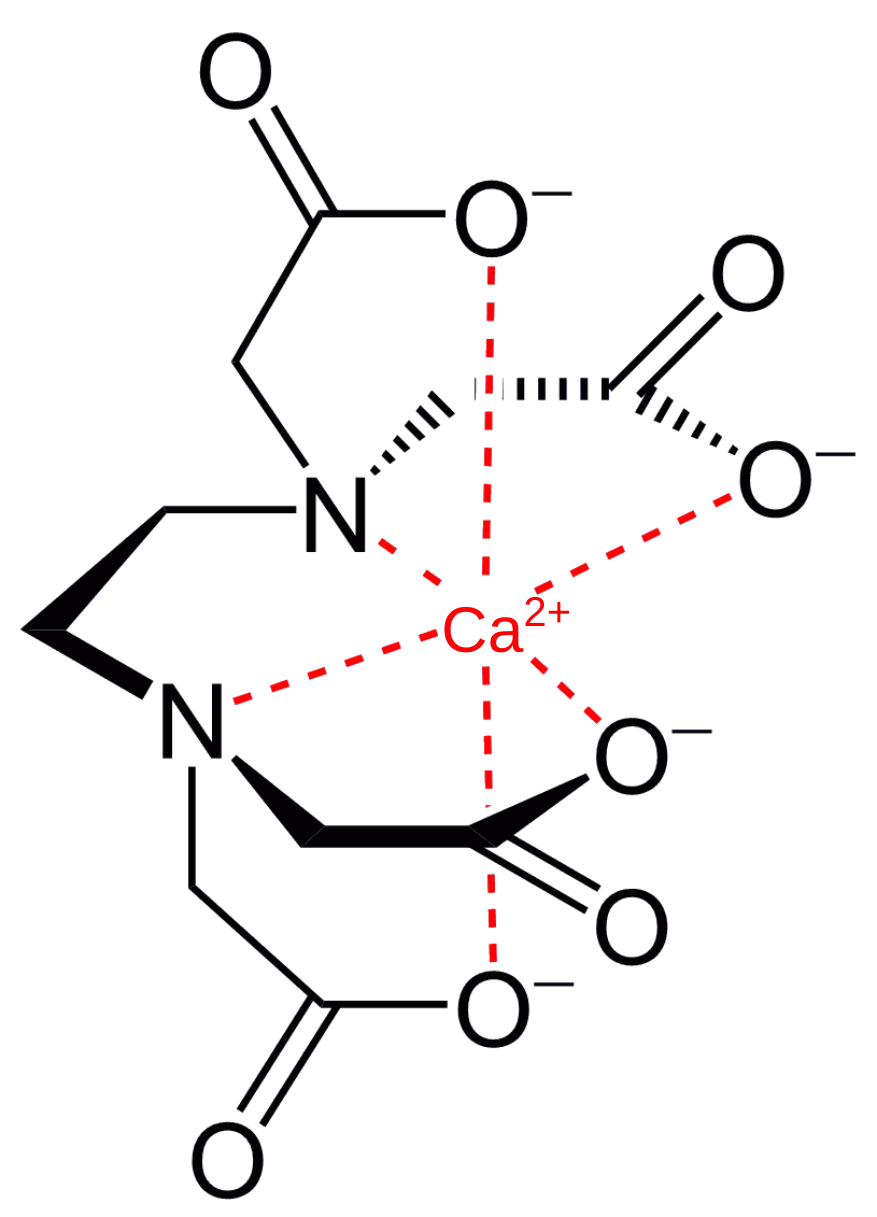
\includegraphics[scale=.6]{ca-edta-komplex.png}
\end{minipage}
\subsubsection{Fehlerbetrachtung} Dem Erlenmaierkolben mit der zu analysierenden Lösung wurde zu viel demineralisiertes Wasser zugegeben. Weitere Fühl- und Messungenauigkeiten sind denkbar, wie z.B. eine verzögerte Reaktion beim Erkennen des Äquivalenzpunktes und dem folgenden Ablesen des titrierten Volumens. \\ 
Die prozentuale Abweichung vom tatsächlichen Wert beträgt:
\begin{equation}
	\frac{4,540\text{ mmol}}{4,514\text{ mmol}} = 0,58 \%
\end{equation}

\section{Literatur}
\begin{enumerate}[label=(\arabic*)]
	\item \emph{Praktische Einführung in die Chemie
für Studierende der Fachrichtungen
Technische Biologie und Physik}. Praktikumsskript, Universität Stuttgart,
SoSe 2017.  
	\item Prof. Dr. D. Gudat. \emph{„Einführung in die Chemie für Naturwissenschaftler“}. Vorlesungsskript
	\item \emph{Das Basiswissen der Chemie}. Charles E. Mortimer, Ulrich Müller. 12. Auflage
	\end{enumerate}
\end{document}		
